\chapter{Inversion Drivers}\label{chapter:ref:Drivers}

Our task in the inversion\index{inversion} is to find the geological structure within a given three-dimensional region $\Omega$ from given geophysical 
observations\index{observation}. 
The structure is described by a \emph{level set function} $m$\index{level set function}.
This function can be a scalar function or may have several components,
see Chapter~\ref{Chp:ref:regularization} for more details.
Its values are dimensionless and should be between zero and one.
However, the latter condition is not enforced.
Through a mapping (see Chapter~\ref{Chp:ref:mapping}\index{mapping}) the values
of the level set function are mapped onto physical parameter $p^f$\index{physical parameter}.
The physical parameter feeds into one or more forward models\index{forward model}
which return a prediction for the observations, see Chapter~\ref{Chp:ref:forward models}.
An inversion may consider several forward models at once which we call
\emph{joint inversion}\index{joint inversion}.


The level set function describing the actual geological structure is given as
the function which minimizes a particular \emph{cost function}
$J$\index{cost function}.
This cost function is a composition of the difference of the predicted
observations to the actual observations for the relevant forward models, and
the regularization term\index{regularization} which controls the smoothness of
the level set function.
In general the cost function $J$ takes the form
\begin{equation}\label{REF:EQU:INTRO 1}
J(m) = J^{reg}(m) + \sum_{f} \mu^{data}_{f} \cdot J^{f}(p^f)
\end{equation} 
where $J^{f}(p)$ is a measure of the defect of the observations predicted for
the parameter $p^f$ against the observations for forward model $f$, and
$J^{reg}(m)$ is the regularization term.
The weighting factors $\mu^{data}_{f}$ are dimensionless, non-negative
trade-off factors\index{trade-off factor}.
Potentially, values for the trade-off factors are altered during the inversion
process in order to improve the balance between the regularization term and
the data defect terms\footnote{The current version does not support an automated selection 
of trade-off factors}.
The physical parameter $p^f$ depends on the level set function
$m$ in a known form:
\begin{equation}\label{REF:EQU:INTRO 1b}
p^f = M_{f}(m)
\end{equation} 
where $M_f$ is a given mapping. For the case of gravity inversion
the $M_f$ is a simple linear function mapping the level set function $m$ with dimensionless values 
to physical density anomaly values $\rho$.
(see Chapter~\ref{Chp:ref:mapping}\index{mapping}). In its simplest from the mapping is given as 
$\rho = \rho_0 \cdot m$ where $\rho_0$ is a reference density. It is pointed out that 
the inversion techniques applied do not constrain limits to the values of the level set function
although there is the notion that its values are between zero and one. However, 
limits can be enforced to physical parameters using appropriate mappings.

The level set function $m$ and consequently the physical parameters $p^f$ are 
defined over a three dimensional domain $\Omega$ which represented by an \escript 
\class{Domain} object, see \cite{ESCRIPT}. The domain builder methods provide 
functions to build appropriate domains from field data sets, see Section~\ref{Chp:ref:domain builder}.
In general the domain is a rectangular three-dimensional domain where the third dimension $x_2=z$ represents
depth. The $z=0$ surface defines the surface of the earth where $z<0$ is defining the subsurface region and
$z>0$ is defining the region above the surface, see Figure~\ref{fig:cartesianDomain}. In general physical parameters such as
density and susceptibility anomaly are known above the surface, typically assumed to be zero. 
For subregions where a physical parameter is known it is assumed that the corresponding level set function as 
the value zero. If required, non-zero values for the physical parameters can be set using appropriate mapping.      

\begin{figure}[ht]
    \centering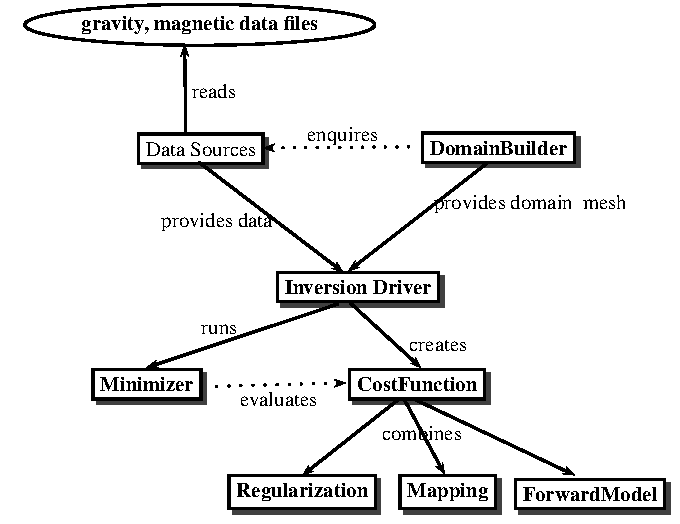
\includegraphics{classdep}
    \caption{Class dependencies}
    \label{fig:classes}
\end{figure} 

\section{Class Dependencies}
For simplification of usage \downunder provides predefined classes that drive inversion for particular 
problems. The usage of this classes is being discussed in Part~\ref{part1}. More details are shown in
Section~\ref{chapter:ref:Drivers:Drivers}. It is the role of the driver class to orchestration an 
inversion. New inversions can easily be implemented by modifying the available drivers.

As illustrated in Figure~\ref{fig:classes} the driver class uses geophysical data as
managed through the \class{DataSource} class (see Chapter~\ref{Chp:ref:data sources}) and 
an \escript domain to define an appropriate
costs function to be minimized. The driver class also run the minimization solver.
The \escript domain~\cite{ESCRIPT} is created using the \class{DomainBuilder}, see Chapter~\ref{Chp:ref:domain builder},
which builds an appropriate domain and mesh based on the geophysical data used in the inversion. 
\class{ReferenceSystem} defines the coordinate system to be used. 
Based on the inversion to be performed (gravity, magnetic, joint) the 
driver class builds an appropriate cost function $J$ including the regularization term $J^{reg}$, see
\class{Regularization} class in Chapter~\ref{Chp:ref:regularization}, 
the forward models, see Chapter~\ref{Chp:ref:forward models} and
the required mappings, see \class{Mapping} class in Chapter~\ref{Chp:ref:mapping},
to connect the level set function with physical parameters. Finally the driver class calls the
solver to minimize the cost function, see Chapter~\ref{chapter:ref:Minimization}.

The driver classes cover commonly used cases for the convenience of users. In fact, 
more general cases can be implemented in an easy way. Script \examplefile{nodriver.py} is an example 
on how to implement an inversion without using one of the driver classes.   








\chapter{Inversion Drivers and Costs Functions}\label{chapter:ref:Drivers}

\begin{classdesc}{SimpleCostFunction}{regularization, mapping, forwardmodel}
    This is a simple cost function with a single continuous (mapped) variable.
    It is the sum of two weighted terms, a single forward model and a single
    regularization term. This cost function is used by the provided gravity
    and magnetic inversion implementations.
\end{classdesc}








 
